\section{Test: Linear model} \label{sec:test_lin}
The purpose of this chapter is to show and discuss the performance results of the LQI controller derived in \cref{sec:ctrl-design} on the linear model derived in \cref{sec:linear_model}. The controller is benchmarked against the original FLC controller with regards to both rotor speed control and fore-aft movement dampening capability. Prior to the test the LQI controller has been tuned such that a satisfactory performance was achieved in VTS.

It is expected that the LQI controller will perform much better in damping the fore-aft movement than the original FLC PI controller. % It is also expected to perform better in generator speed control despite the fact that the original FLC controller has been tuned to achieve the best possible generator speed tracking performance. The reason for this prediction might be less obvious. The reason is that the LQI controller has been tuned on the simple linear model and not in VTS like the FLC PI controller. Thus potential unforeseen consequences of having an aggressive controller in a more realistic environment are not discovered until it is tested in VTS.

Test results are shown for both frequency and time domain.


\subsection{Test framework}
Matlab is used to make bode plots and Matlab Simulink is used to run time simulations. The Matlab \textit{connect()} function is utilized with component models defined on a specific form to gain transfer functions or state space systems from one or more inputs to one or more outputs. From these the \textit{bode()} Matlab function is used to make bode plots. 

Time simulations are made with the FLC PI and LQI controlled linear models from the $ A $, $ B $ and $ C $ system matrices and controller gains $ K $. In \cref{fig:simulink_setup2} the Simulink simulation setup is seen. Two systems are observed with the top one containing the original FLC PI controller without FATD enabled and the bottom one being the one with the designed LQI controller. While not directly apparent because of the missing state feedback, the top system is a closed loop system with the controller gain $ K $ contained in the $ A $ and $ B $ matrix. The reason for this is simply that the FLC component described in \cref{sec:comp_flc} is defined as a generic component model and conveniently combined with the Matlab \textit{connect()} function to yield a full closed-loop system.

From the left the free wind disturbance deviation from the operating point is observed entering both systems. The wind data is extracted from VTS simulations and thus mimic the wind turbulence realistically. The simulation is run for a total of 1000 seconds and are initialized at the operating point except for the tower top position $ p_y $ which is initialized with a deviation of 5 m to provoke a response from both systems.
\begin{figure}[ht]
	\centering
	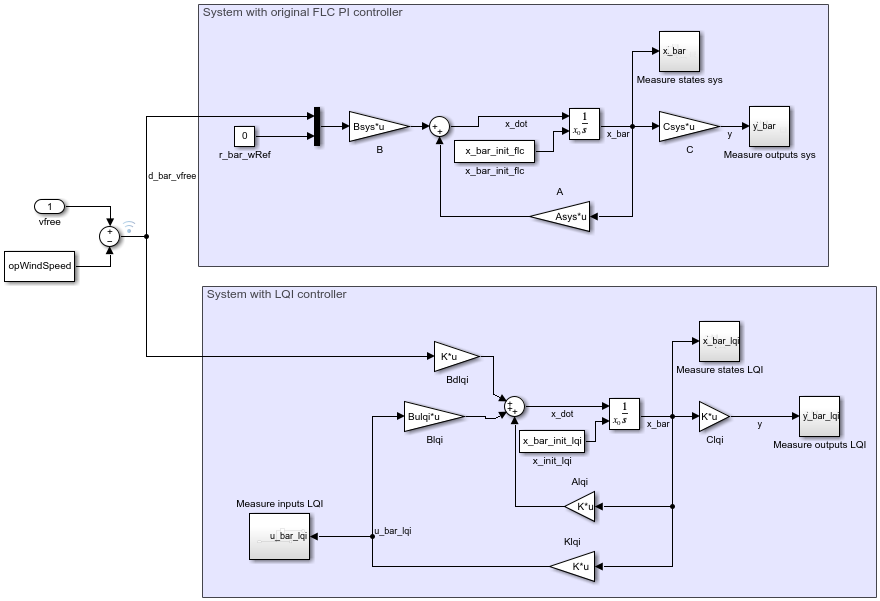
\includegraphics[width=0.95\linewidth]{Graphics/TestResults/linearModPerf/simulink_setup2.png}
	\caption{The Matlab Simulink setup. The free wind speed is observed entering the system from the left.}
	\label{fig:simulink_setup2}
\end{figure}

\subsection{Test results}
In this section the test results are presented and discussed.


\subsubsection{Frequency Domain}
In figure \cref{fig:script_vfreeTovy} the frequency response from the free wind disturbance $ v_{free} $ to the surge direction tower top velocity $ v_y $ is seen. Both the FLC PI system and LQI system are plotted for comparison. As observed in figure \cref{fig:script_vfreeToW} where the frequency response from $ v_{free} $ to $ \Omega $ is seen the LQI controller yields much greater dampening of the eigenfrequency than the FLC PI controller.
\begin{figure}[ht]
	\centering
	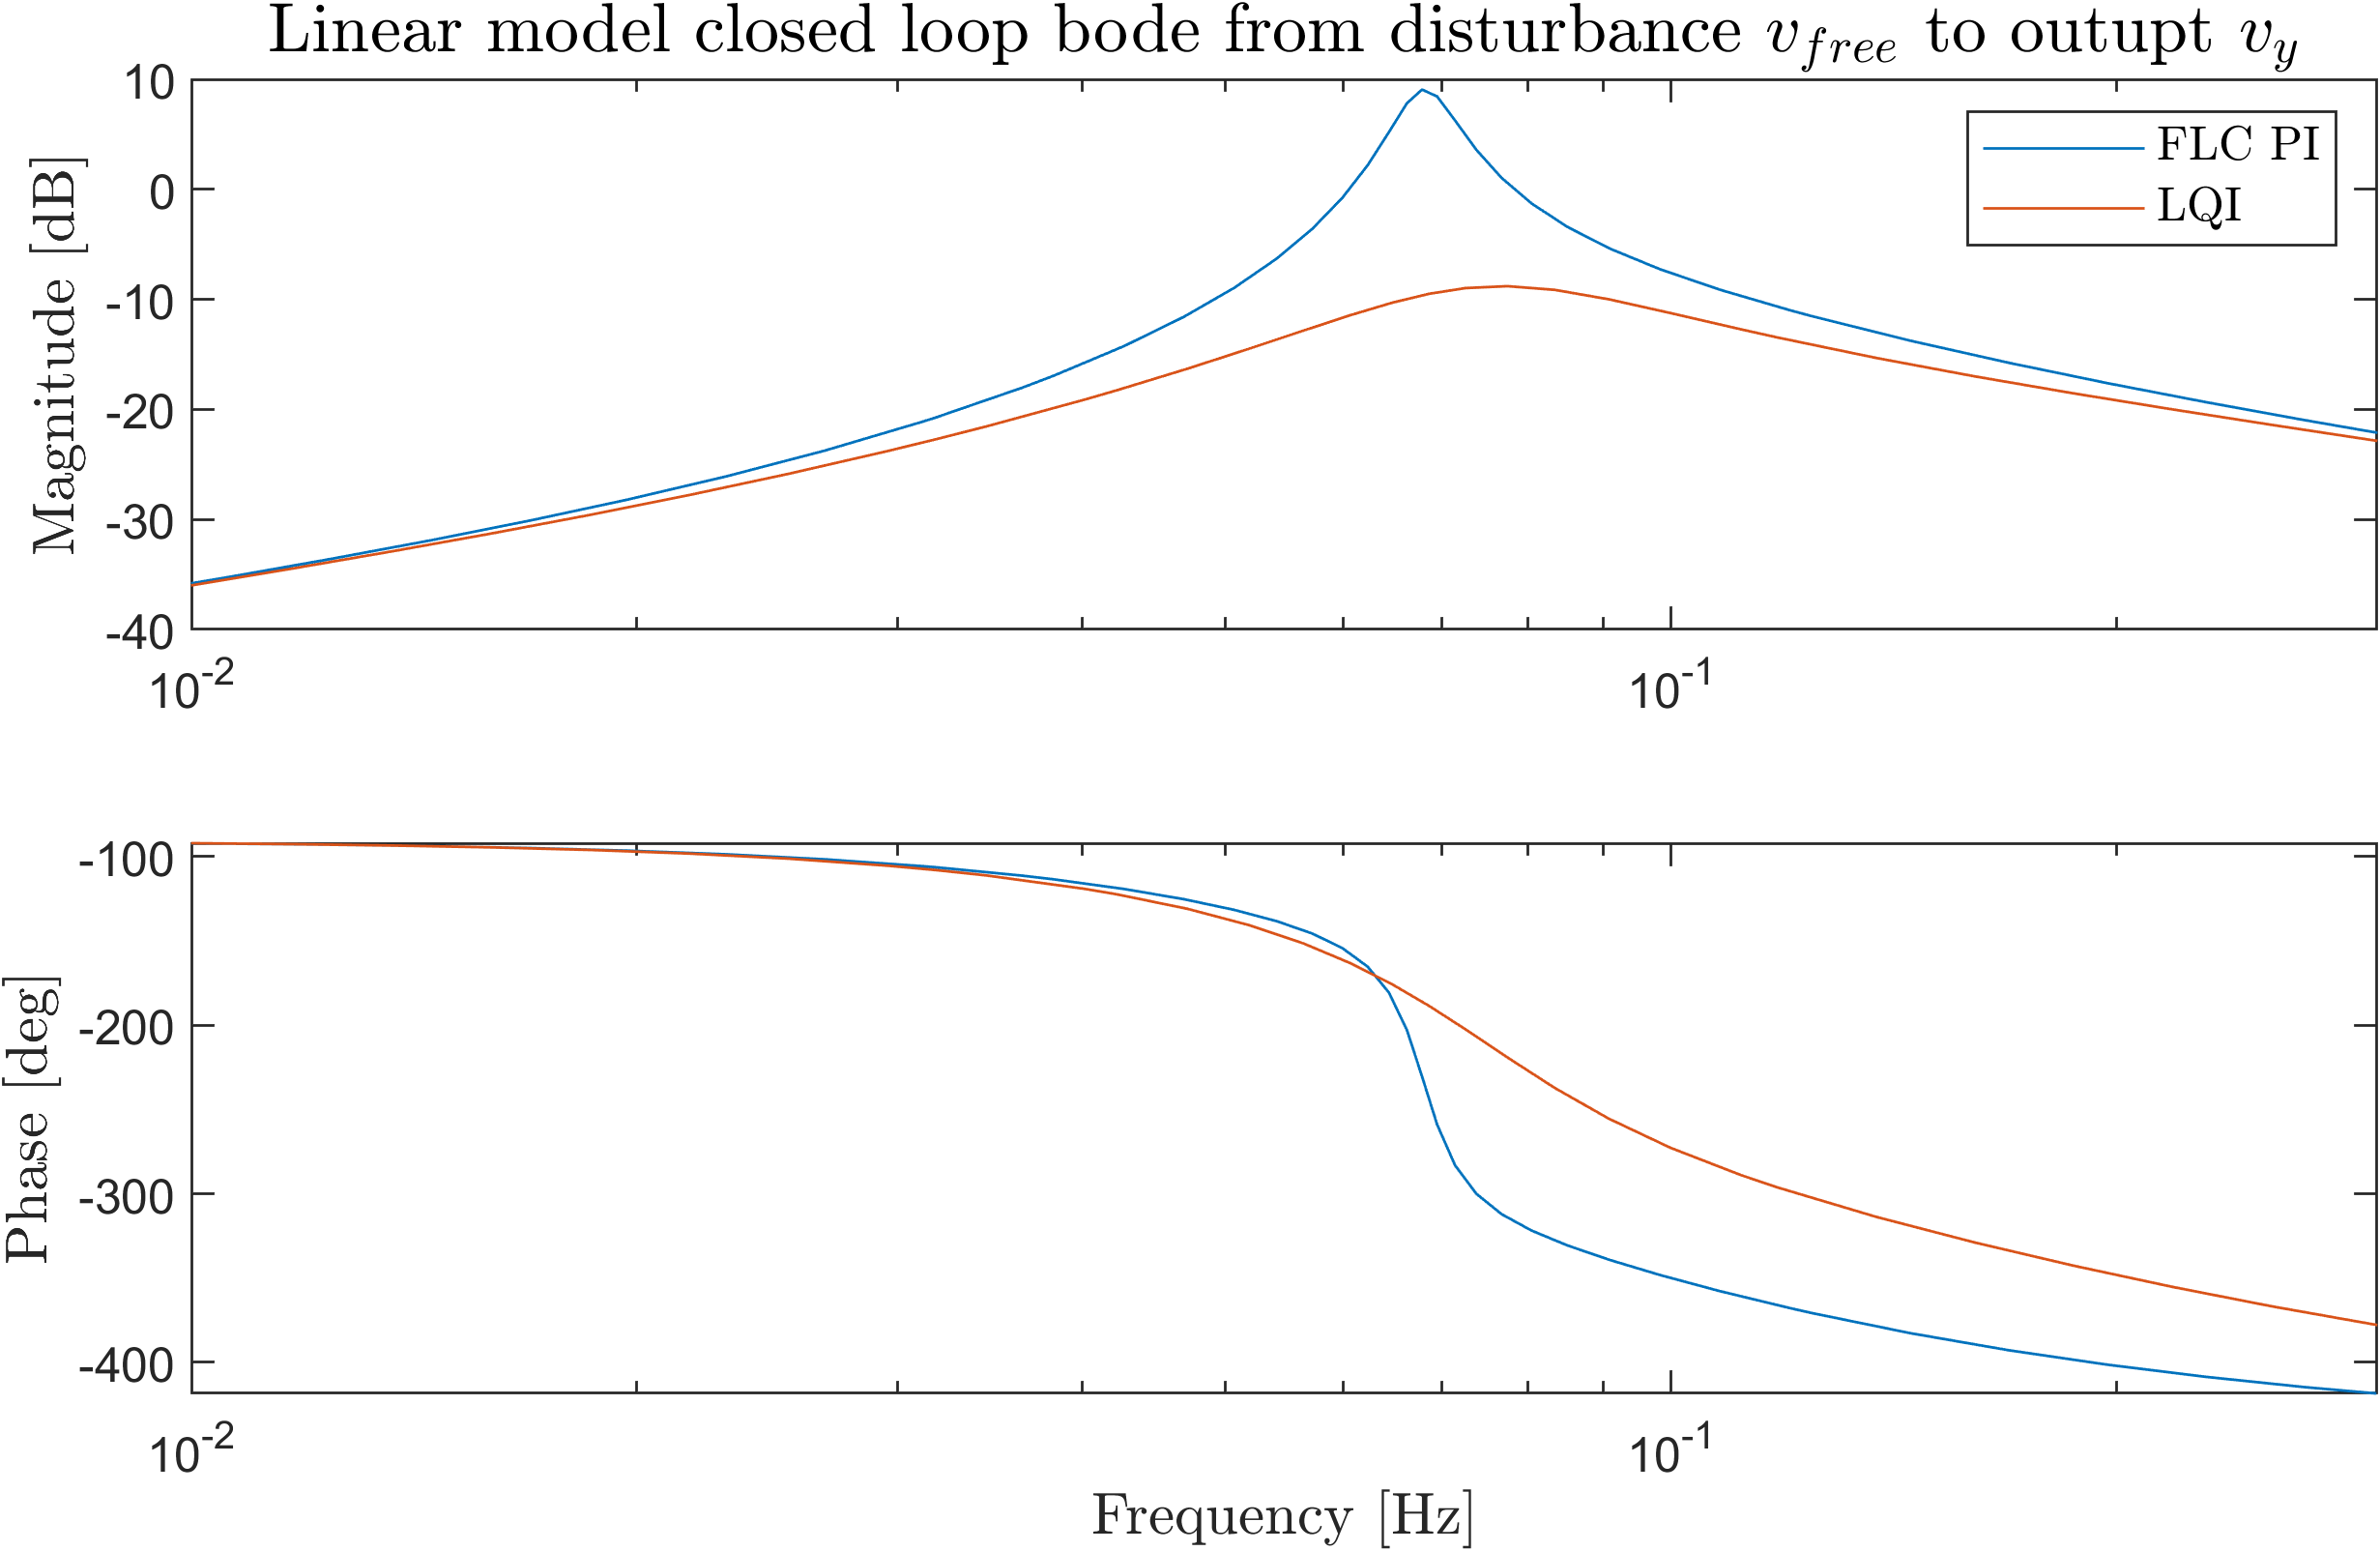
\includegraphics[width=0.7\linewidth]{Graphics/TestResults/linearModPerf/script_vfreeTovy.png}
	\caption{Frequency response from the free wind as observed by the rotor ($ v_{free} $) to the rotor speed  ($ \Omega $) of the linear model with comparison between the original FLC PI controller and the developed LQI controller.}
	\label{fig:script_vfreeTovy}
\end{figure}
 In \cref{fig:script_vfreeTovy} where the frequency response from $ v_{free} $ to $ v_y $ is plotted the same tendency is observed. The LQI controller furthermore dampens the magintude around 4-7 dB more than the FLC PI controller before the eigenfrequency around 0.035 Hz. It also dampens the magnitude more after the eigenfrequency but decreasingly for higher frequencies.
\begin{figure}[ht]
	\centering
	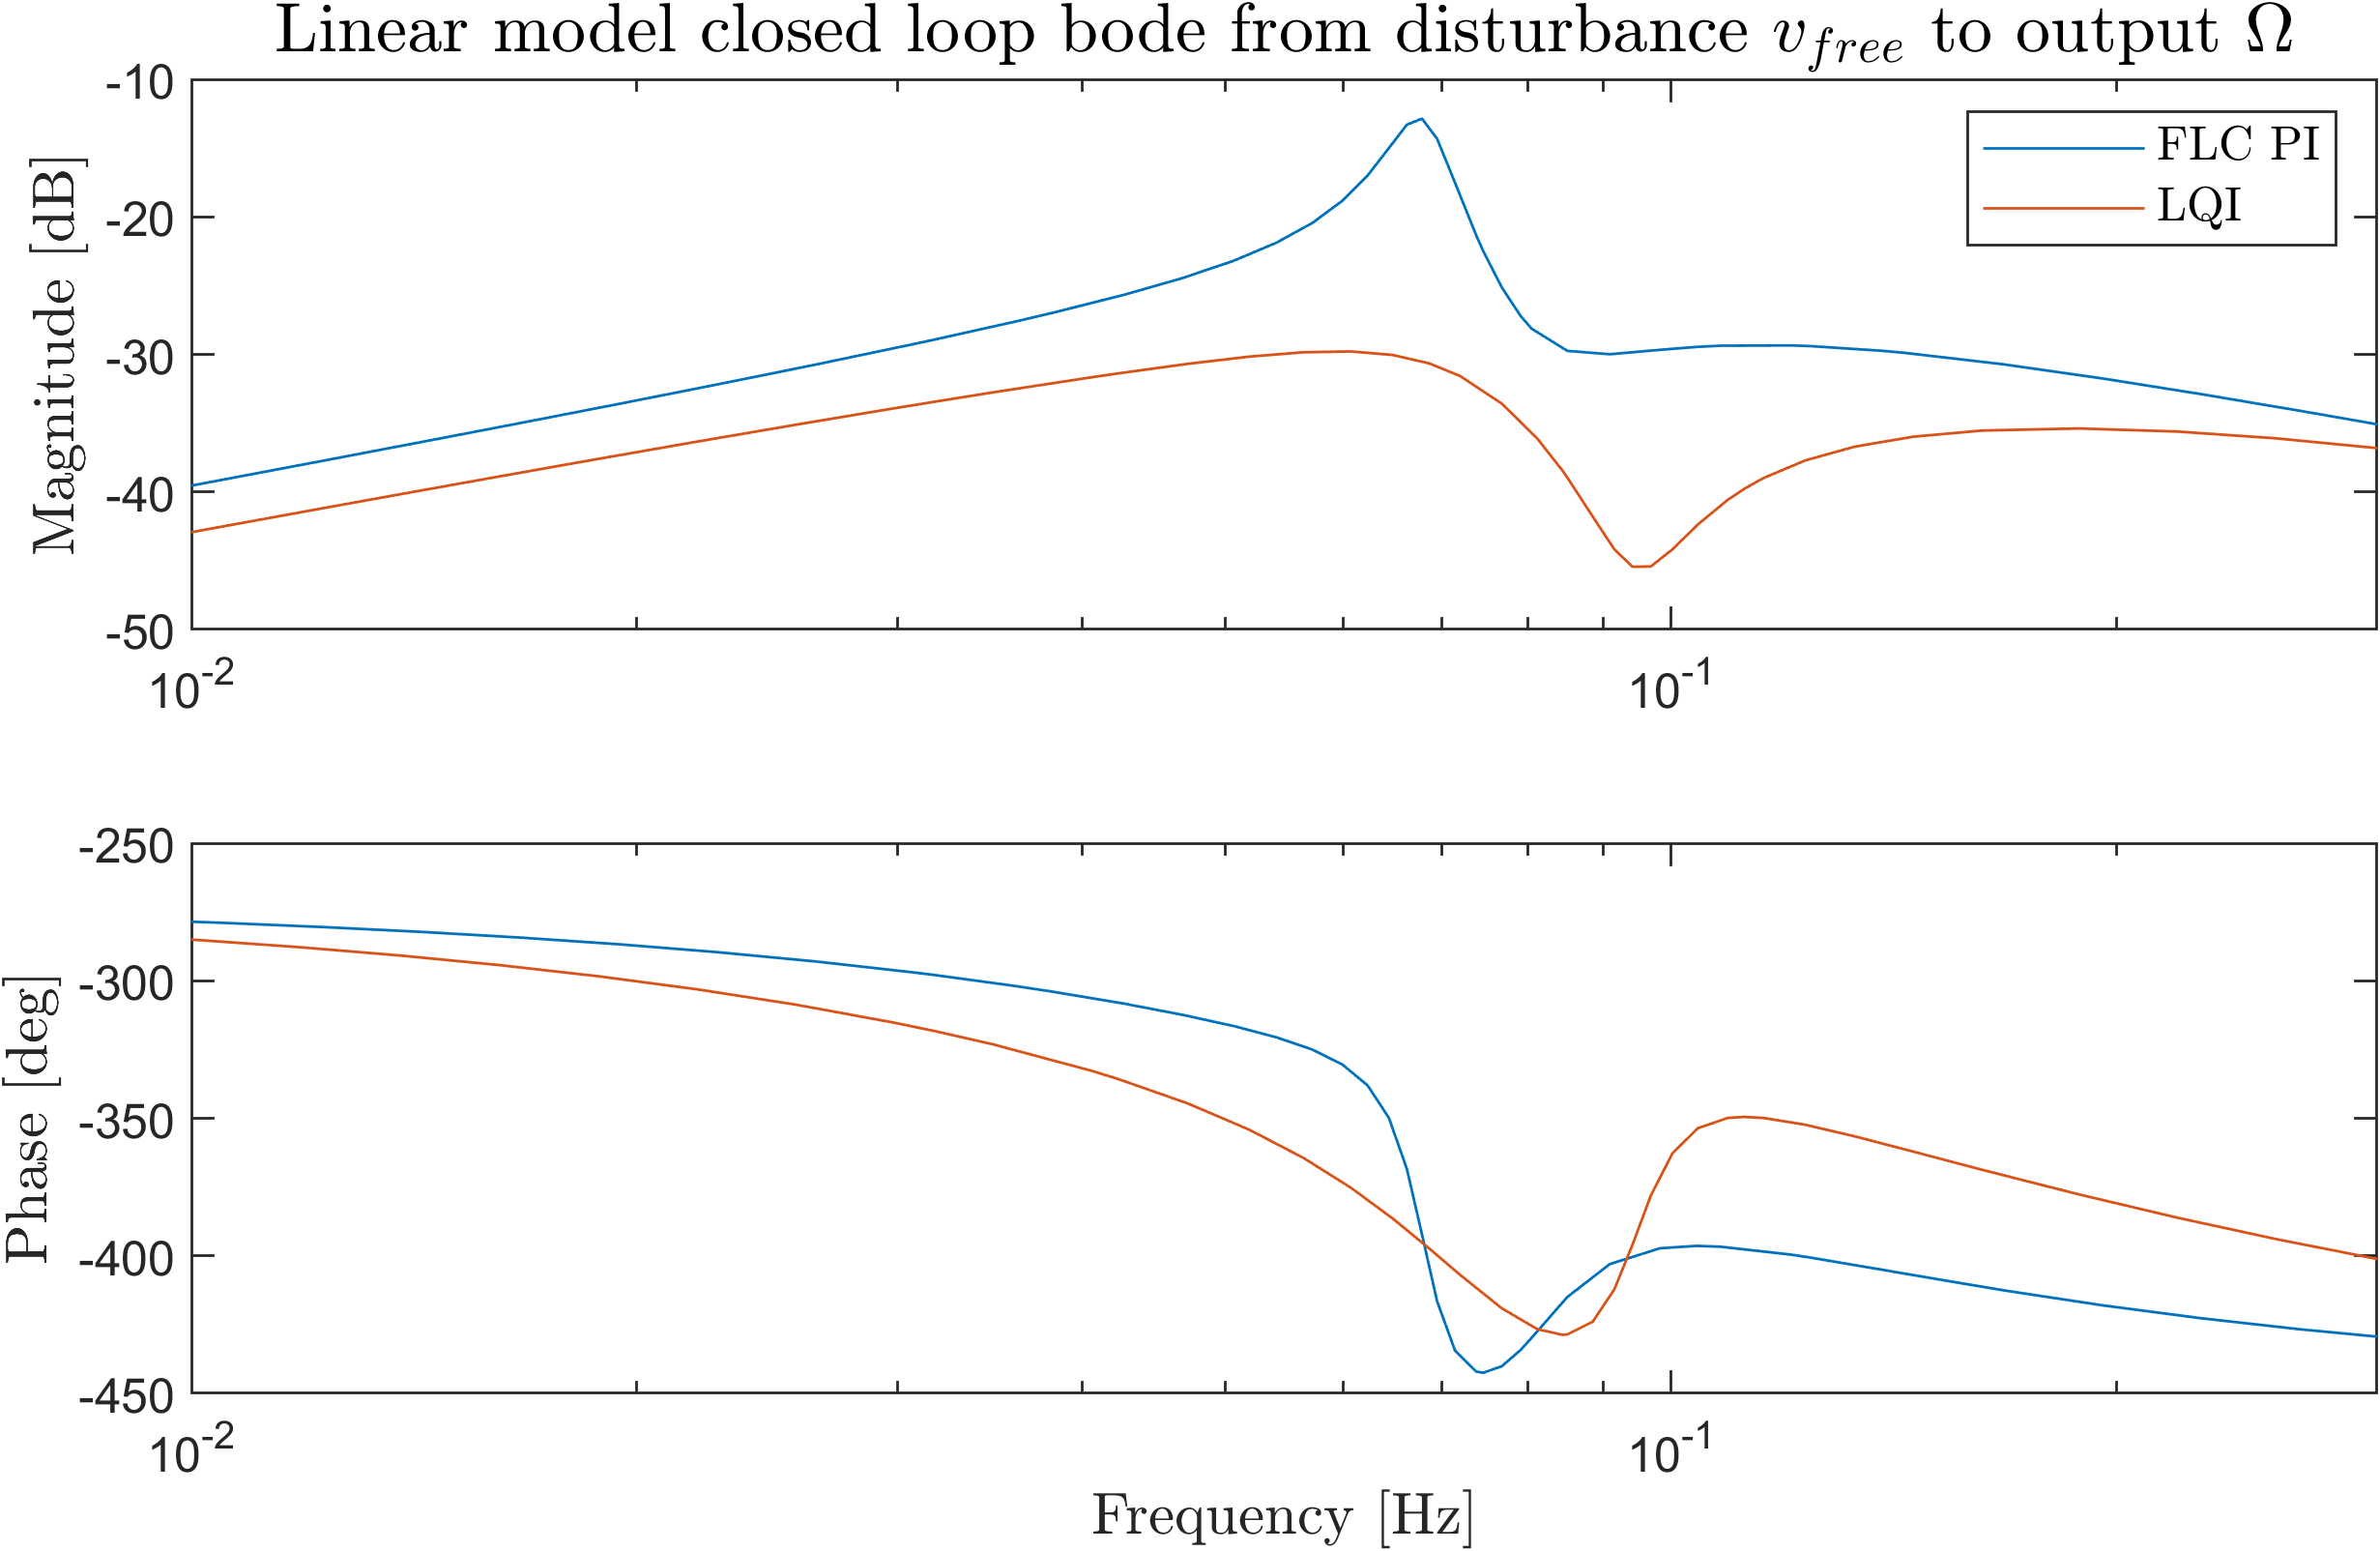
\includegraphics[width=0.7\linewidth]{Graphics/TestResults/linearModPerf/script_vfreeToW.png}
	\caption{Frequency response from the free wind as observed by the rotor ($ v_{free} $) to the surge direction tower top velocity ($ v_y $) of the linear model with comparison between the original FLC PI controller and the developed LQI controller.}
	\label{fig:script_vfreeToW}
\end{figure}
From the frequency responses it can be concluded that the LQI controller will perform better at both rotor speed tracking and fore-aft movement damping. 

\clearpage
\subsubsection{Time domain}
In \cref{fig:sim_11_W_py_vy_comp} the rotor speed, surge direction position and surge direction velocity is plotted. Both the FLC PI and LQI controlled systems are plotted for comparison. Both rotor speed tracking and fore-aft motion performance is vastly superior for the LQI controller. The poor rotor speed tracking performance of the FLC controller is expected because of its lack of consideration for the fore-aft motion. At around 250 to 320 s the fore-aft oscillations are lowered for a while and during this period the rotor speed tracking is improved.
\begin{figure}[ht]
	\centering
	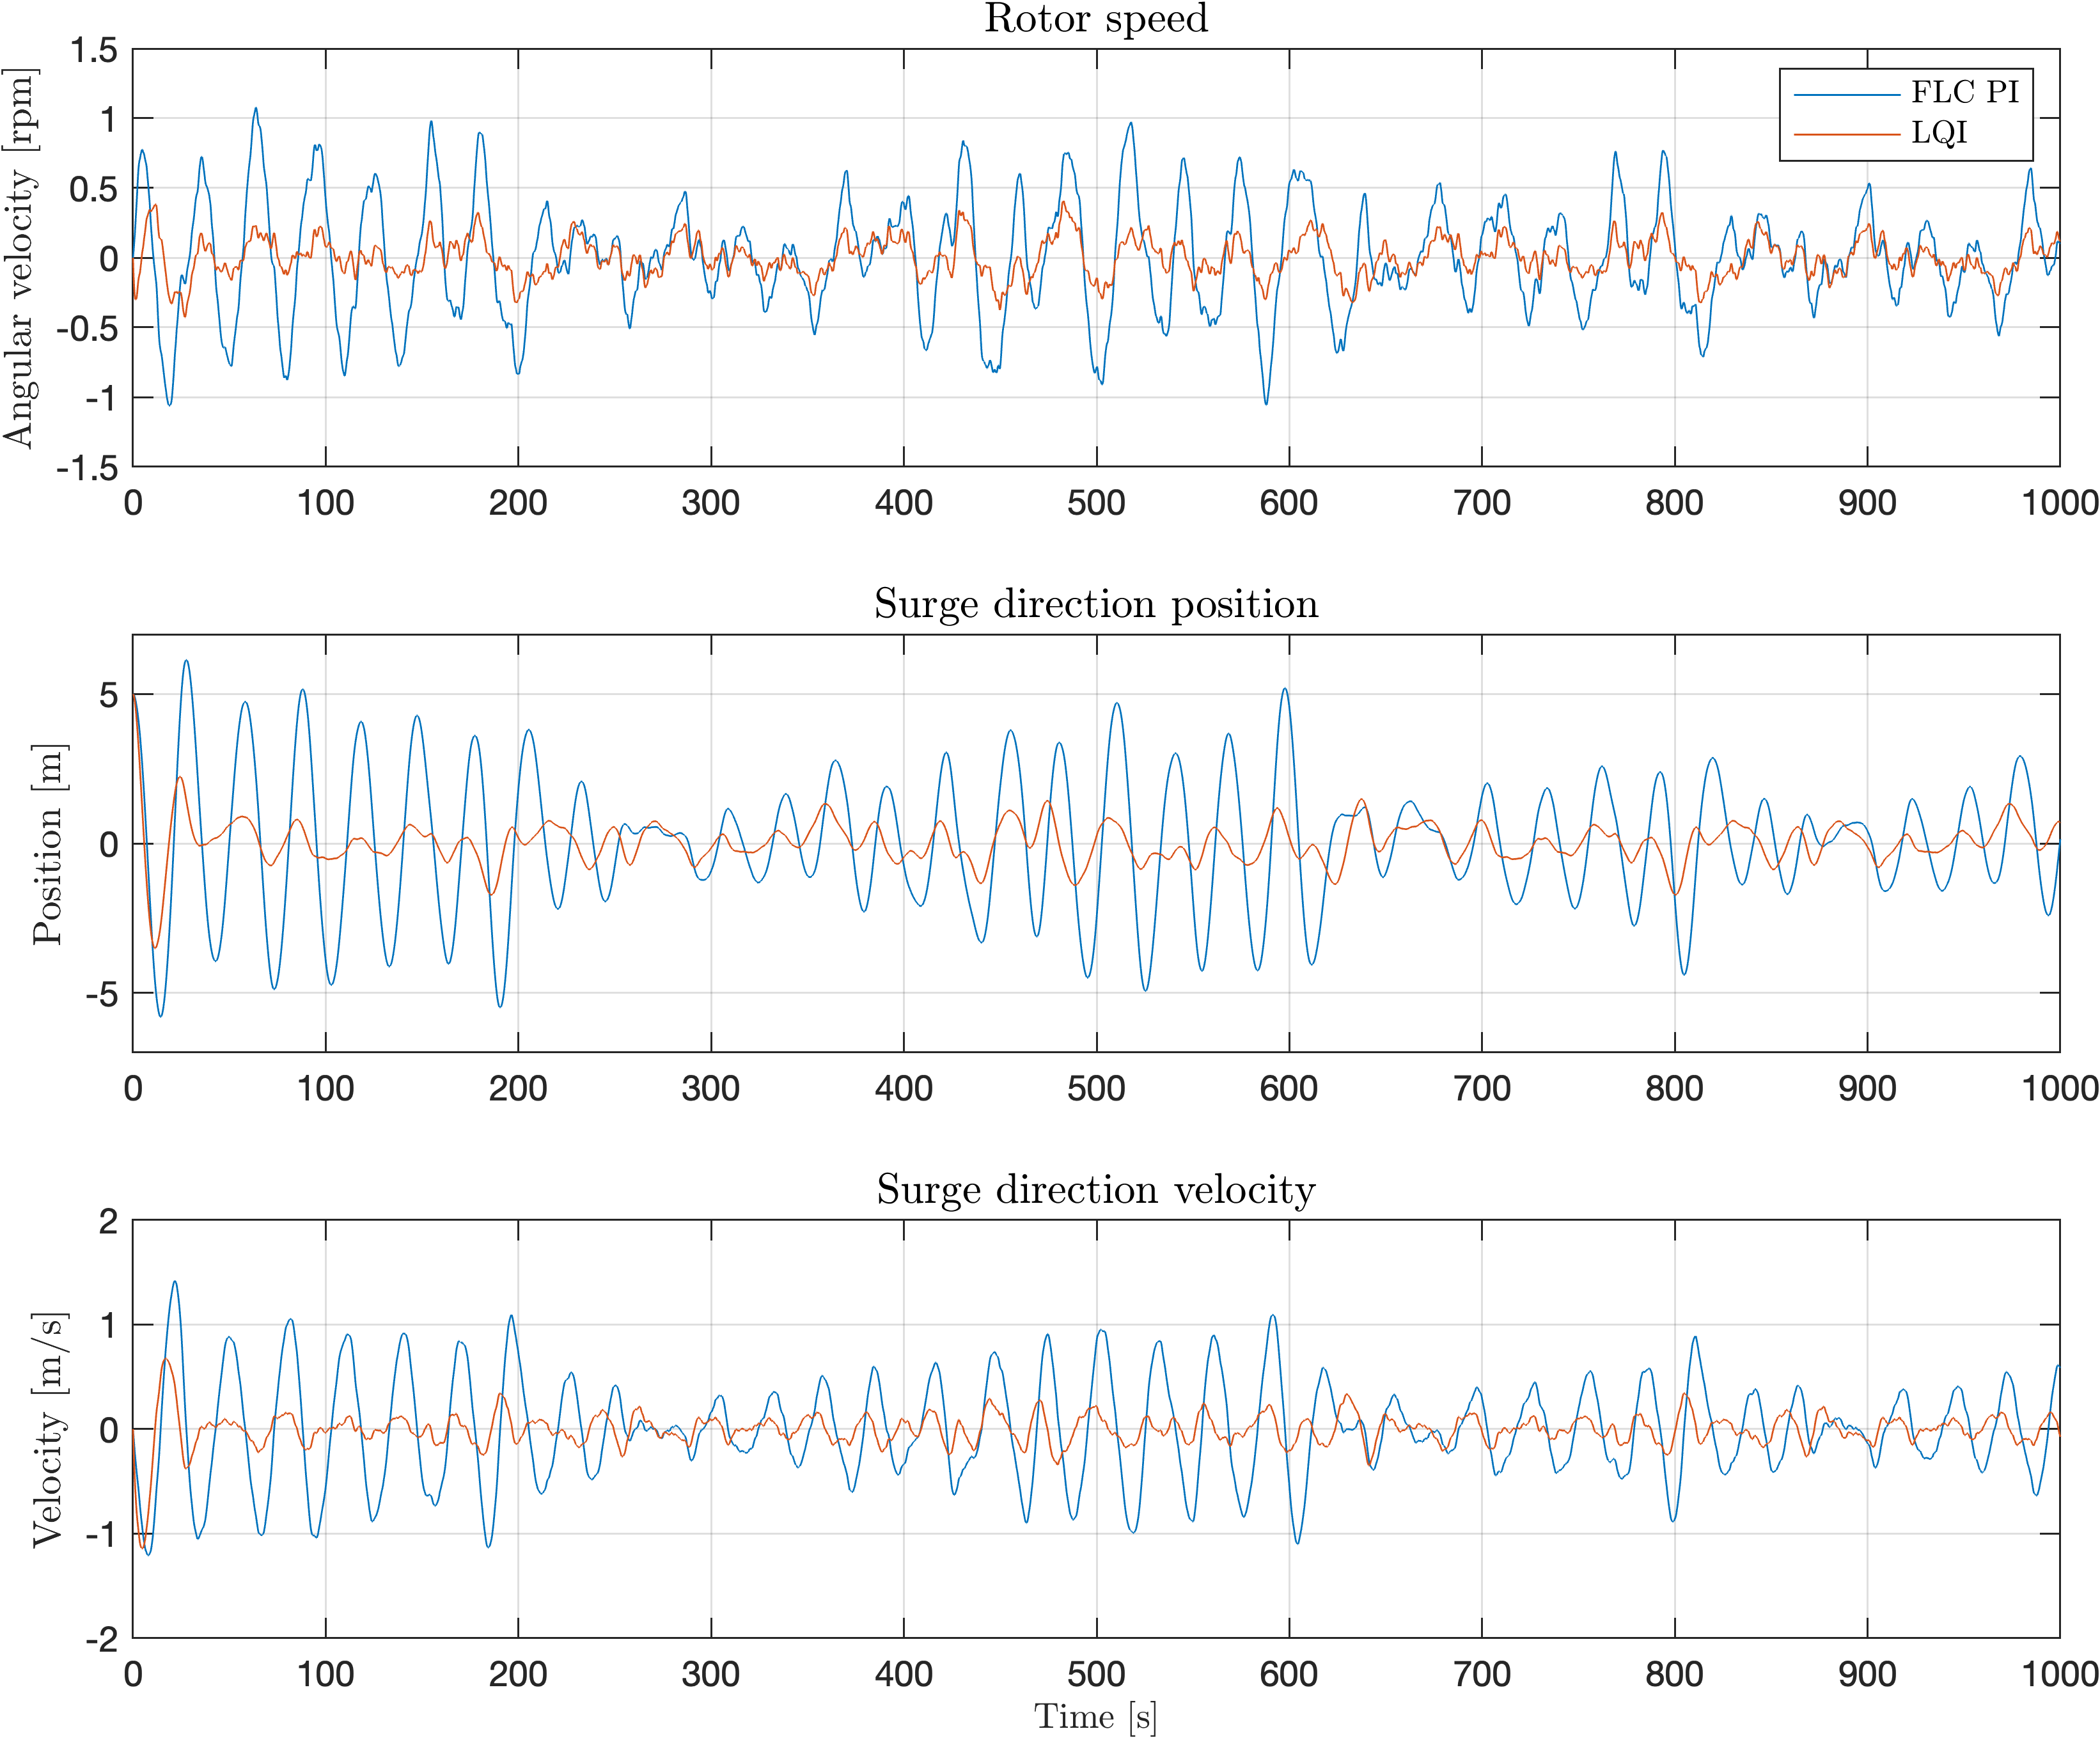
\includegraphics[width=0.7\linewidth]{Graphics/TestResults/linearModPerf/sim_11_W_py_vy_comp.png}
	\caption{Simulink simulation results. The 5 m deviation initialization of the tower top position is visible from the \textit{Surge direction position} at 0 s.}
	\label{fig:sim_11_W_py_vy_comp}
\end{figure}
\cref{fig:sim_12_W_py_vy_comp_zoom} shows a plot zoomed in at the start of the simulation. It is apparent that the LQI controller corrects for the fore-aft position deviation in effectively in 30 to 40 seconds.
\begin{figure}[ht]
	\centering
	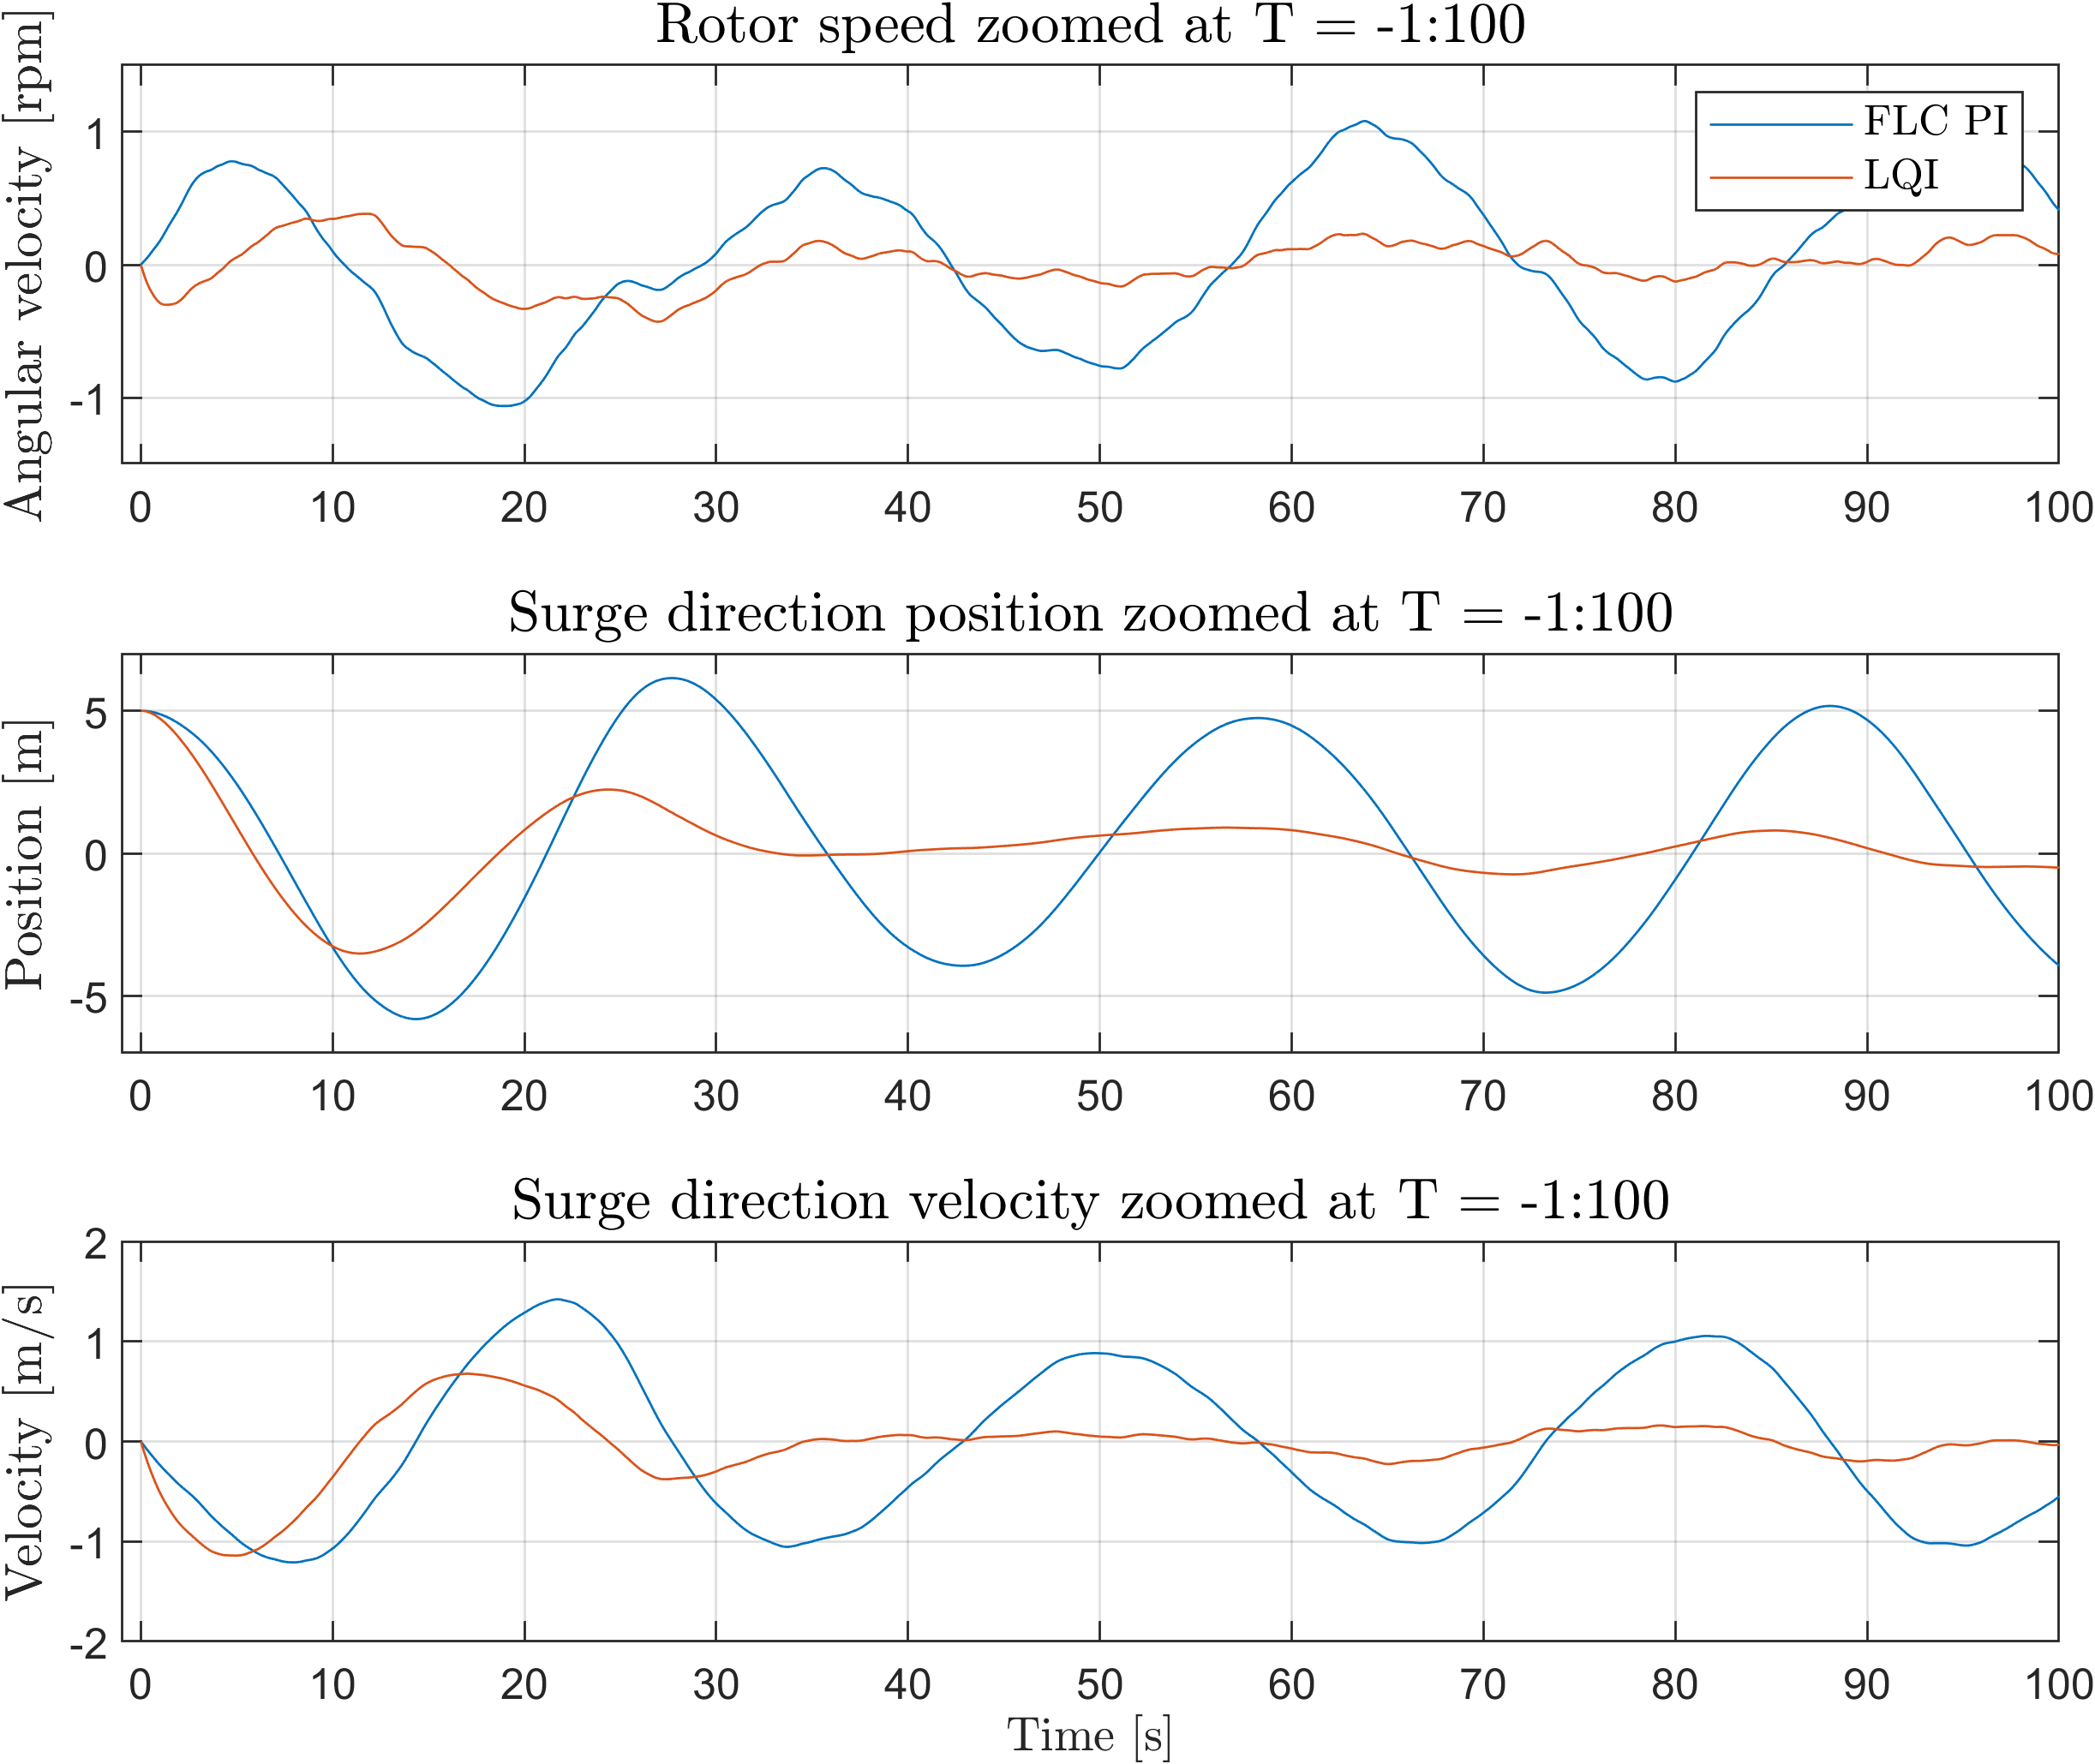
\includegraphics[width=0.7\linewidth]{Graphics/TestResults/linearModPerf/sim_12_W_py_vy_comp_zoom.png}
	\caption{Simulink simulation results zoomed in at the first 100 seconds where the surge direction position is initialized at 5 m.}
	\label{fig:sim_12_W_py_vy_comp_zoom}
\end{figure}
The LQI controller pitch reference deviation from the operating point and its rate of change is plotted in \cref{fig:sim_10_pitch}. Both the absolute value of the pitch reference and its rate of change should not exceed values which are realistic for the wind turbine at the operating point. In the initial transient where the fore-aft position deviates by 5 m the pitch reference starts at 6 degrees and decreases with a rate og change starting at close to -3 deg/s. Neither the rate of change nor the absolute value are deemed problematic especially because such an abrupt change would not occur in a realistic scenario. For the remainder of the simulation the absolute value of the pitch reference deviation stays below 4 deg and the rate of change absolute value stays below 2 deg/s. These values are well inside an acceptable range.
\begin{figure}[ht]
	\centering
	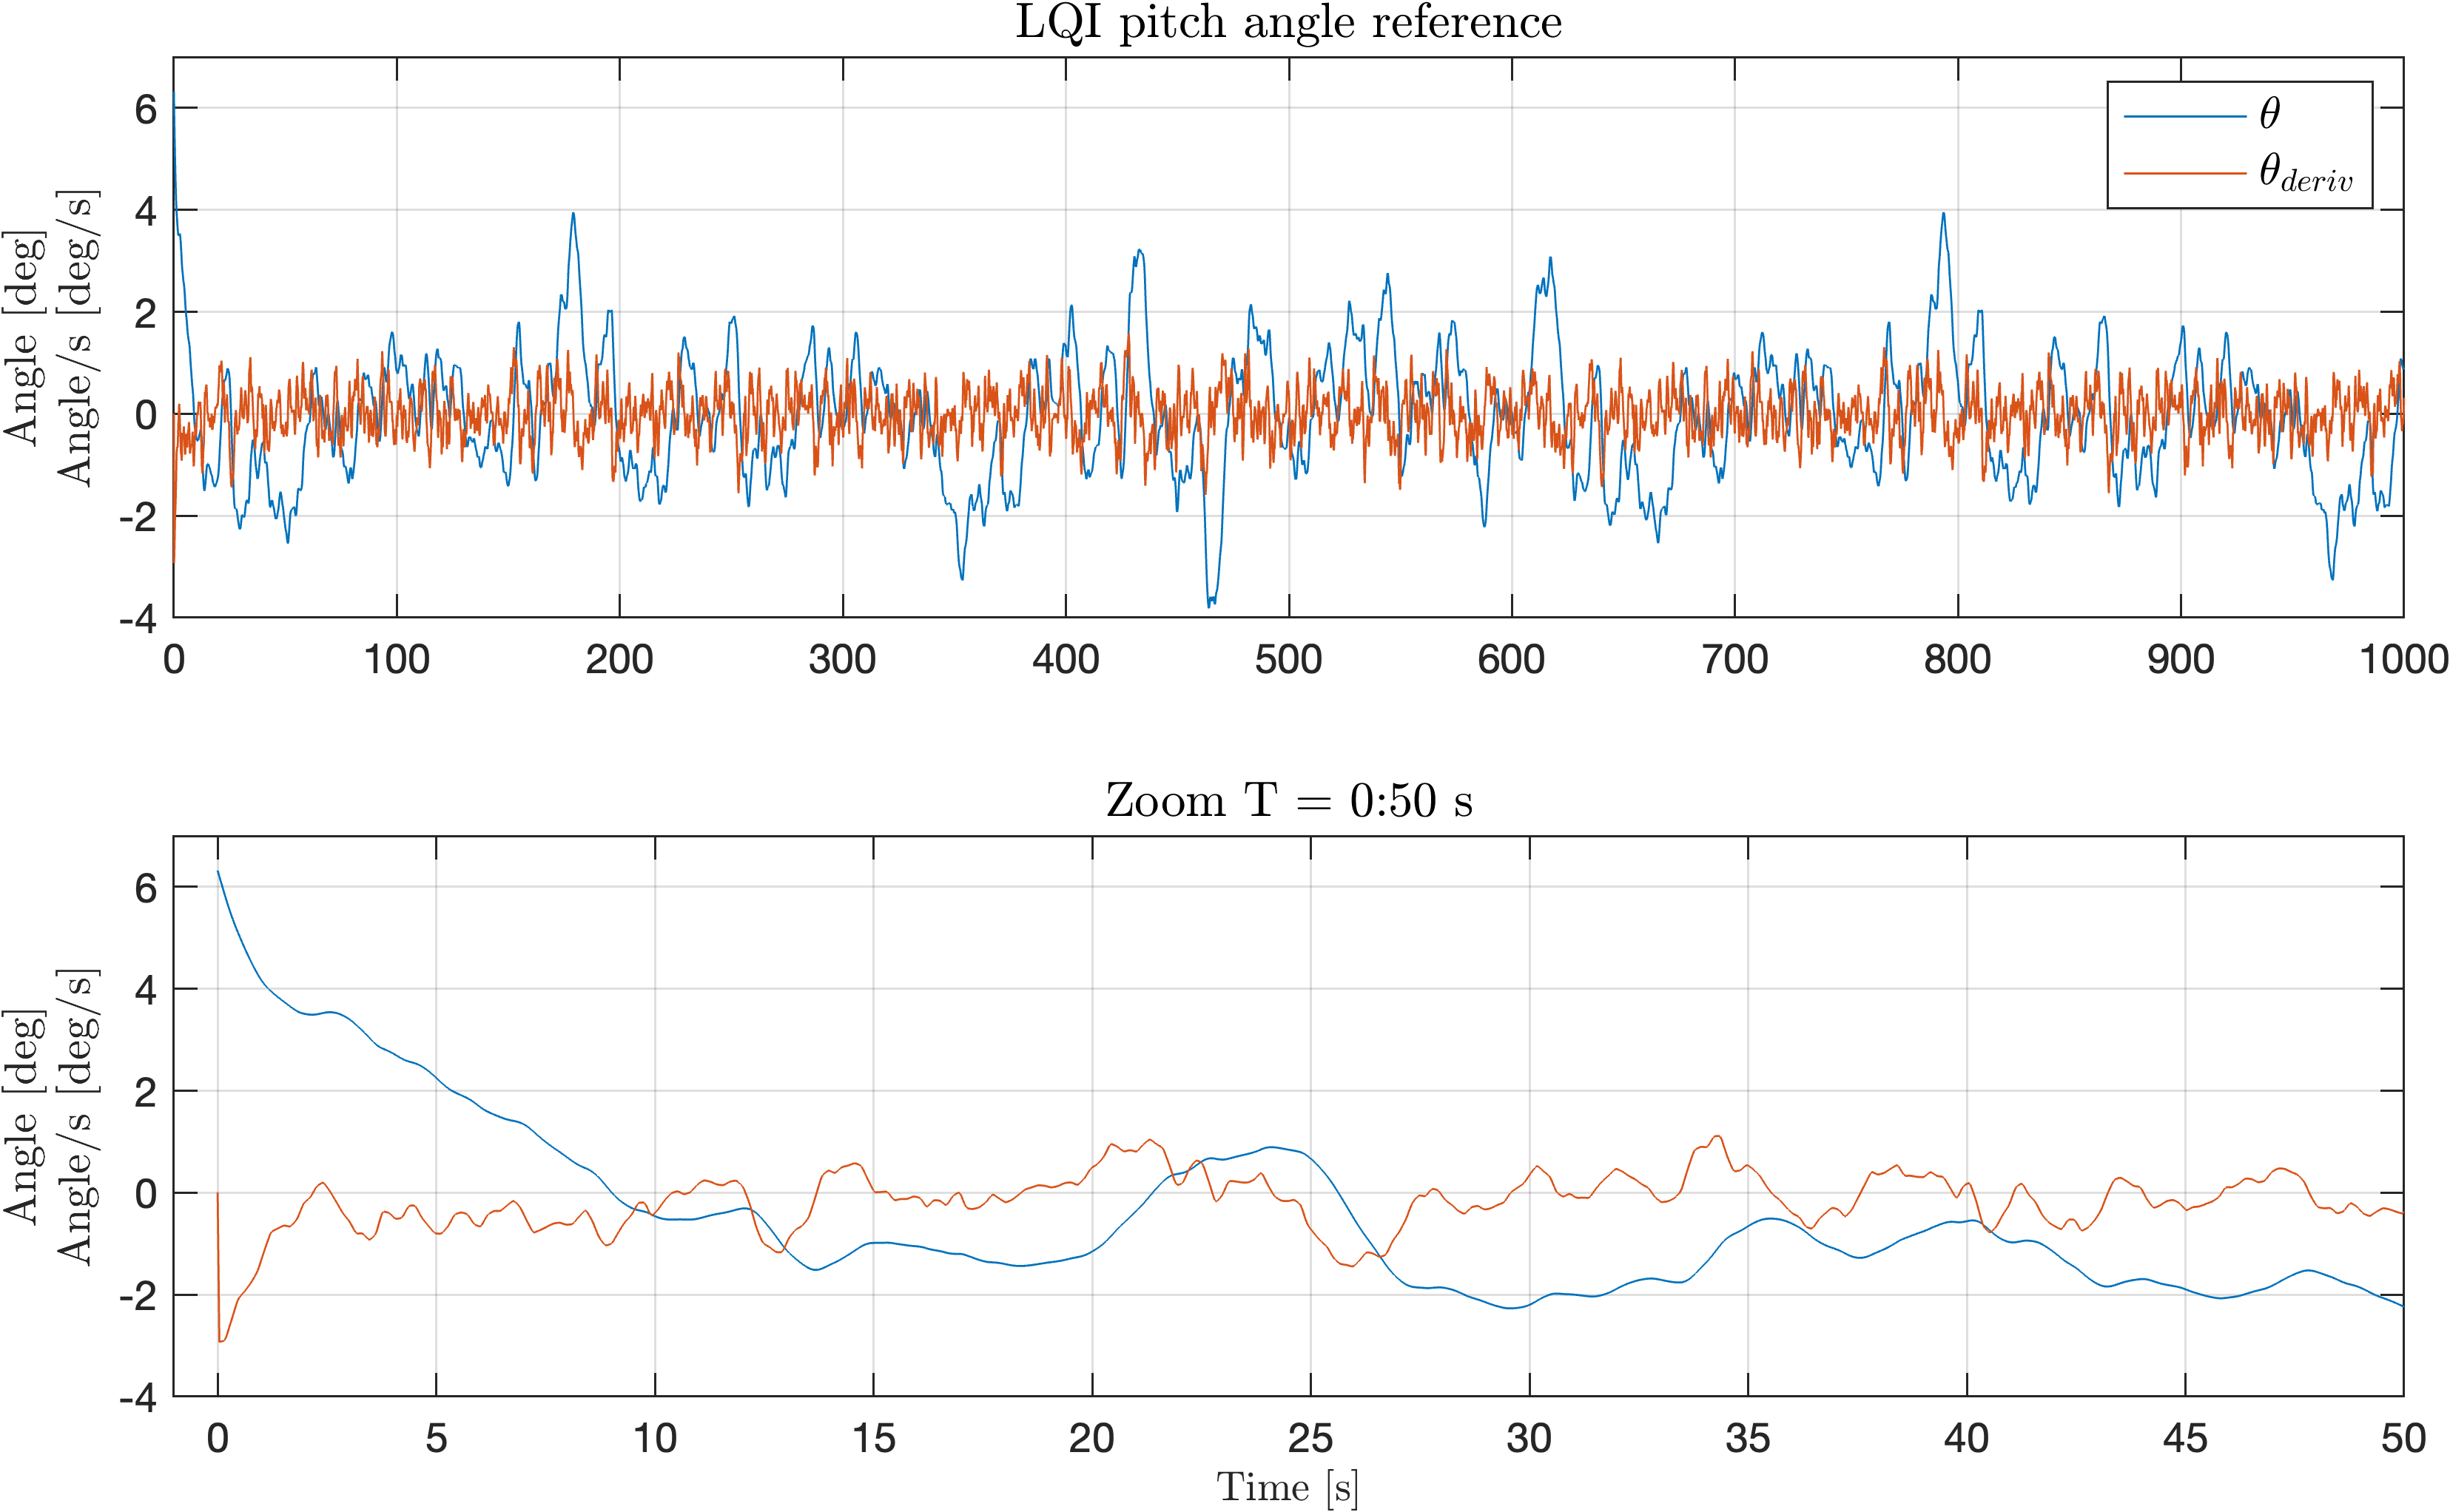
\includegraphics[width=0.7\linewidth]{Graphics/TestResults/linearModPerf/sim_10_pitch.png}
	\caption{Simulink simulation results of the pitch reference and pitch reference change. It is important that neither the absolute value of the pirch reference nor the change in pitch reference exceed realistic values.}
	\label{fig:sim_10_pitch}
\end{figure}

Conclusively the LQI controller performance is very good on the linear model in comparison to the FLC PI controller. This is also to be expected given the...


% OLD PLOTS WITH vfree STEP
%\begin{figure}[ht]
%	\centering
%	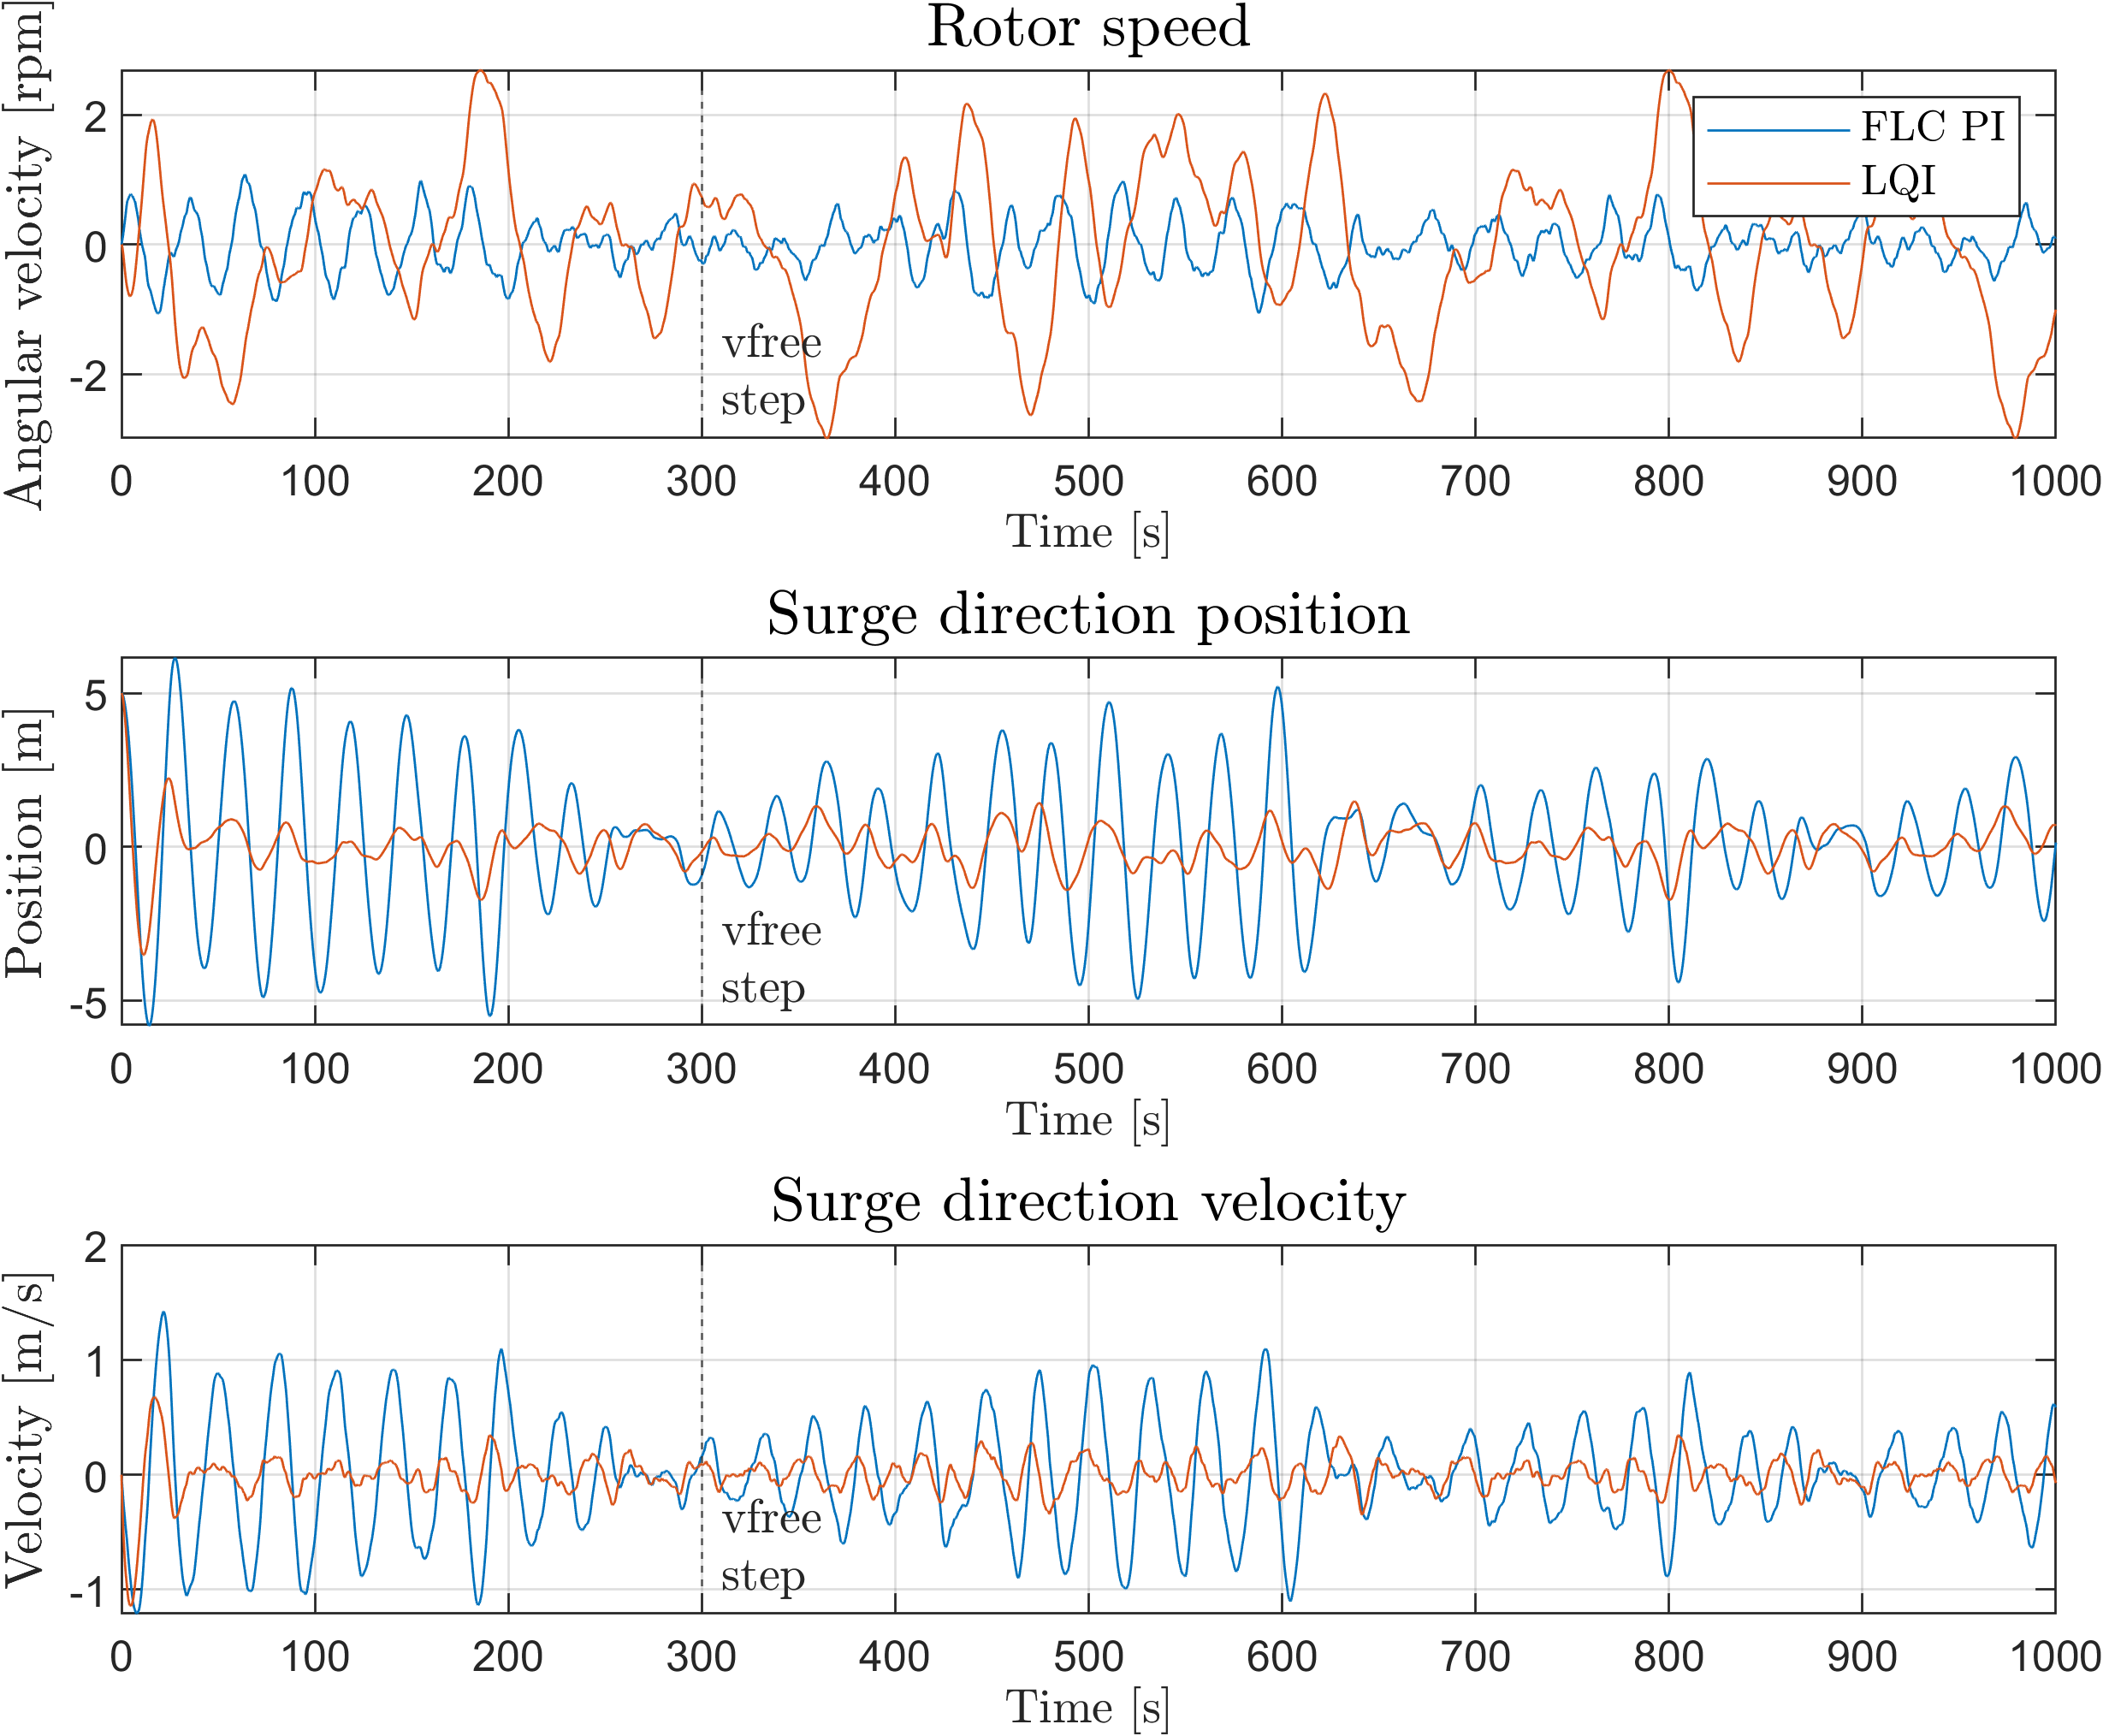
\includegraphics[width=0.7\linewidth]{Graphics/TestResults/linearModPerf/sim_02_W_py_vy_comp.png}
%	\caption{Simulink simulation results. The 10 m deviation initialization of the tower top position is visible from the \textit{Surge direction position} at 0 s.}
%	\label{fig:sim_02_W_py_vy_comp}
%\end{figure}
%
%\begin{figure}[ht]
%	\centering
%	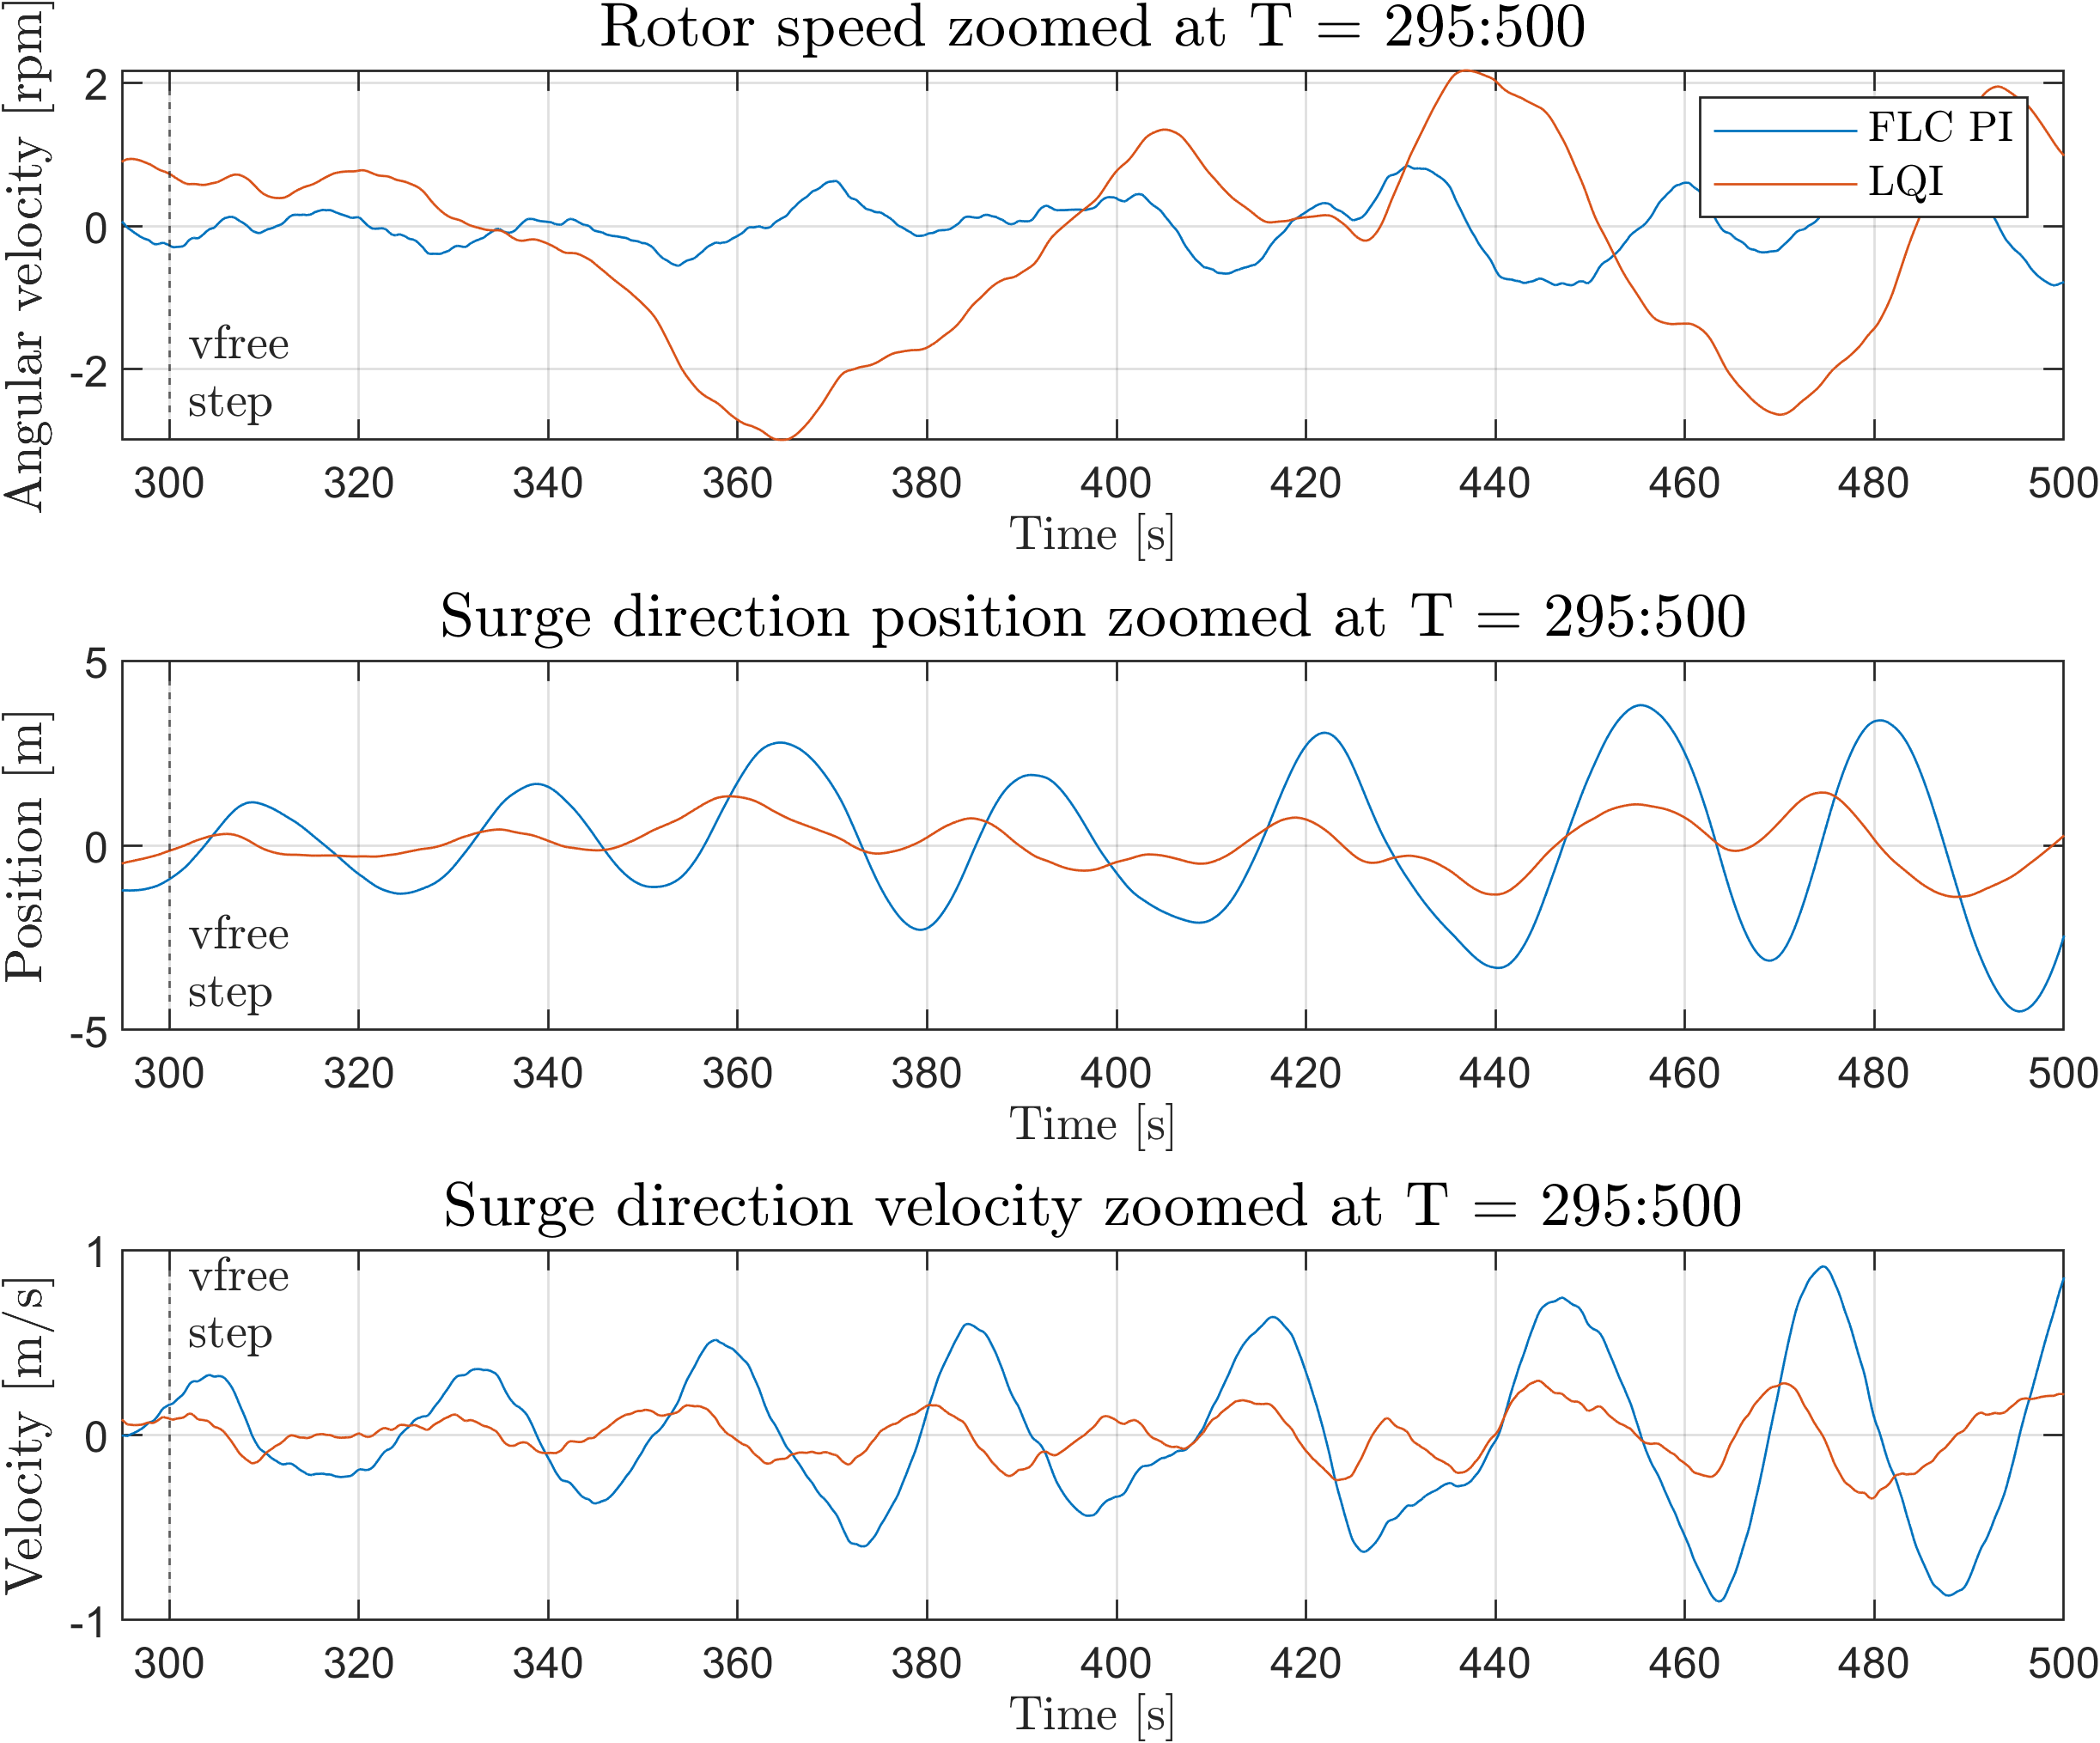
\includegraphics[width=0.7\linewidth]{Graphics/TestResults/linearModPerf/sim_03_W_py_vy_comp_zoom.png}
%	\caption{Simulink simulation results. Zoom at the disturbance step.}
%	\label{fig:sim_03_W_py_vy_comp_zoom}
%\end{figure}
%
%\begin{figure}[ht]
%	\centering
%	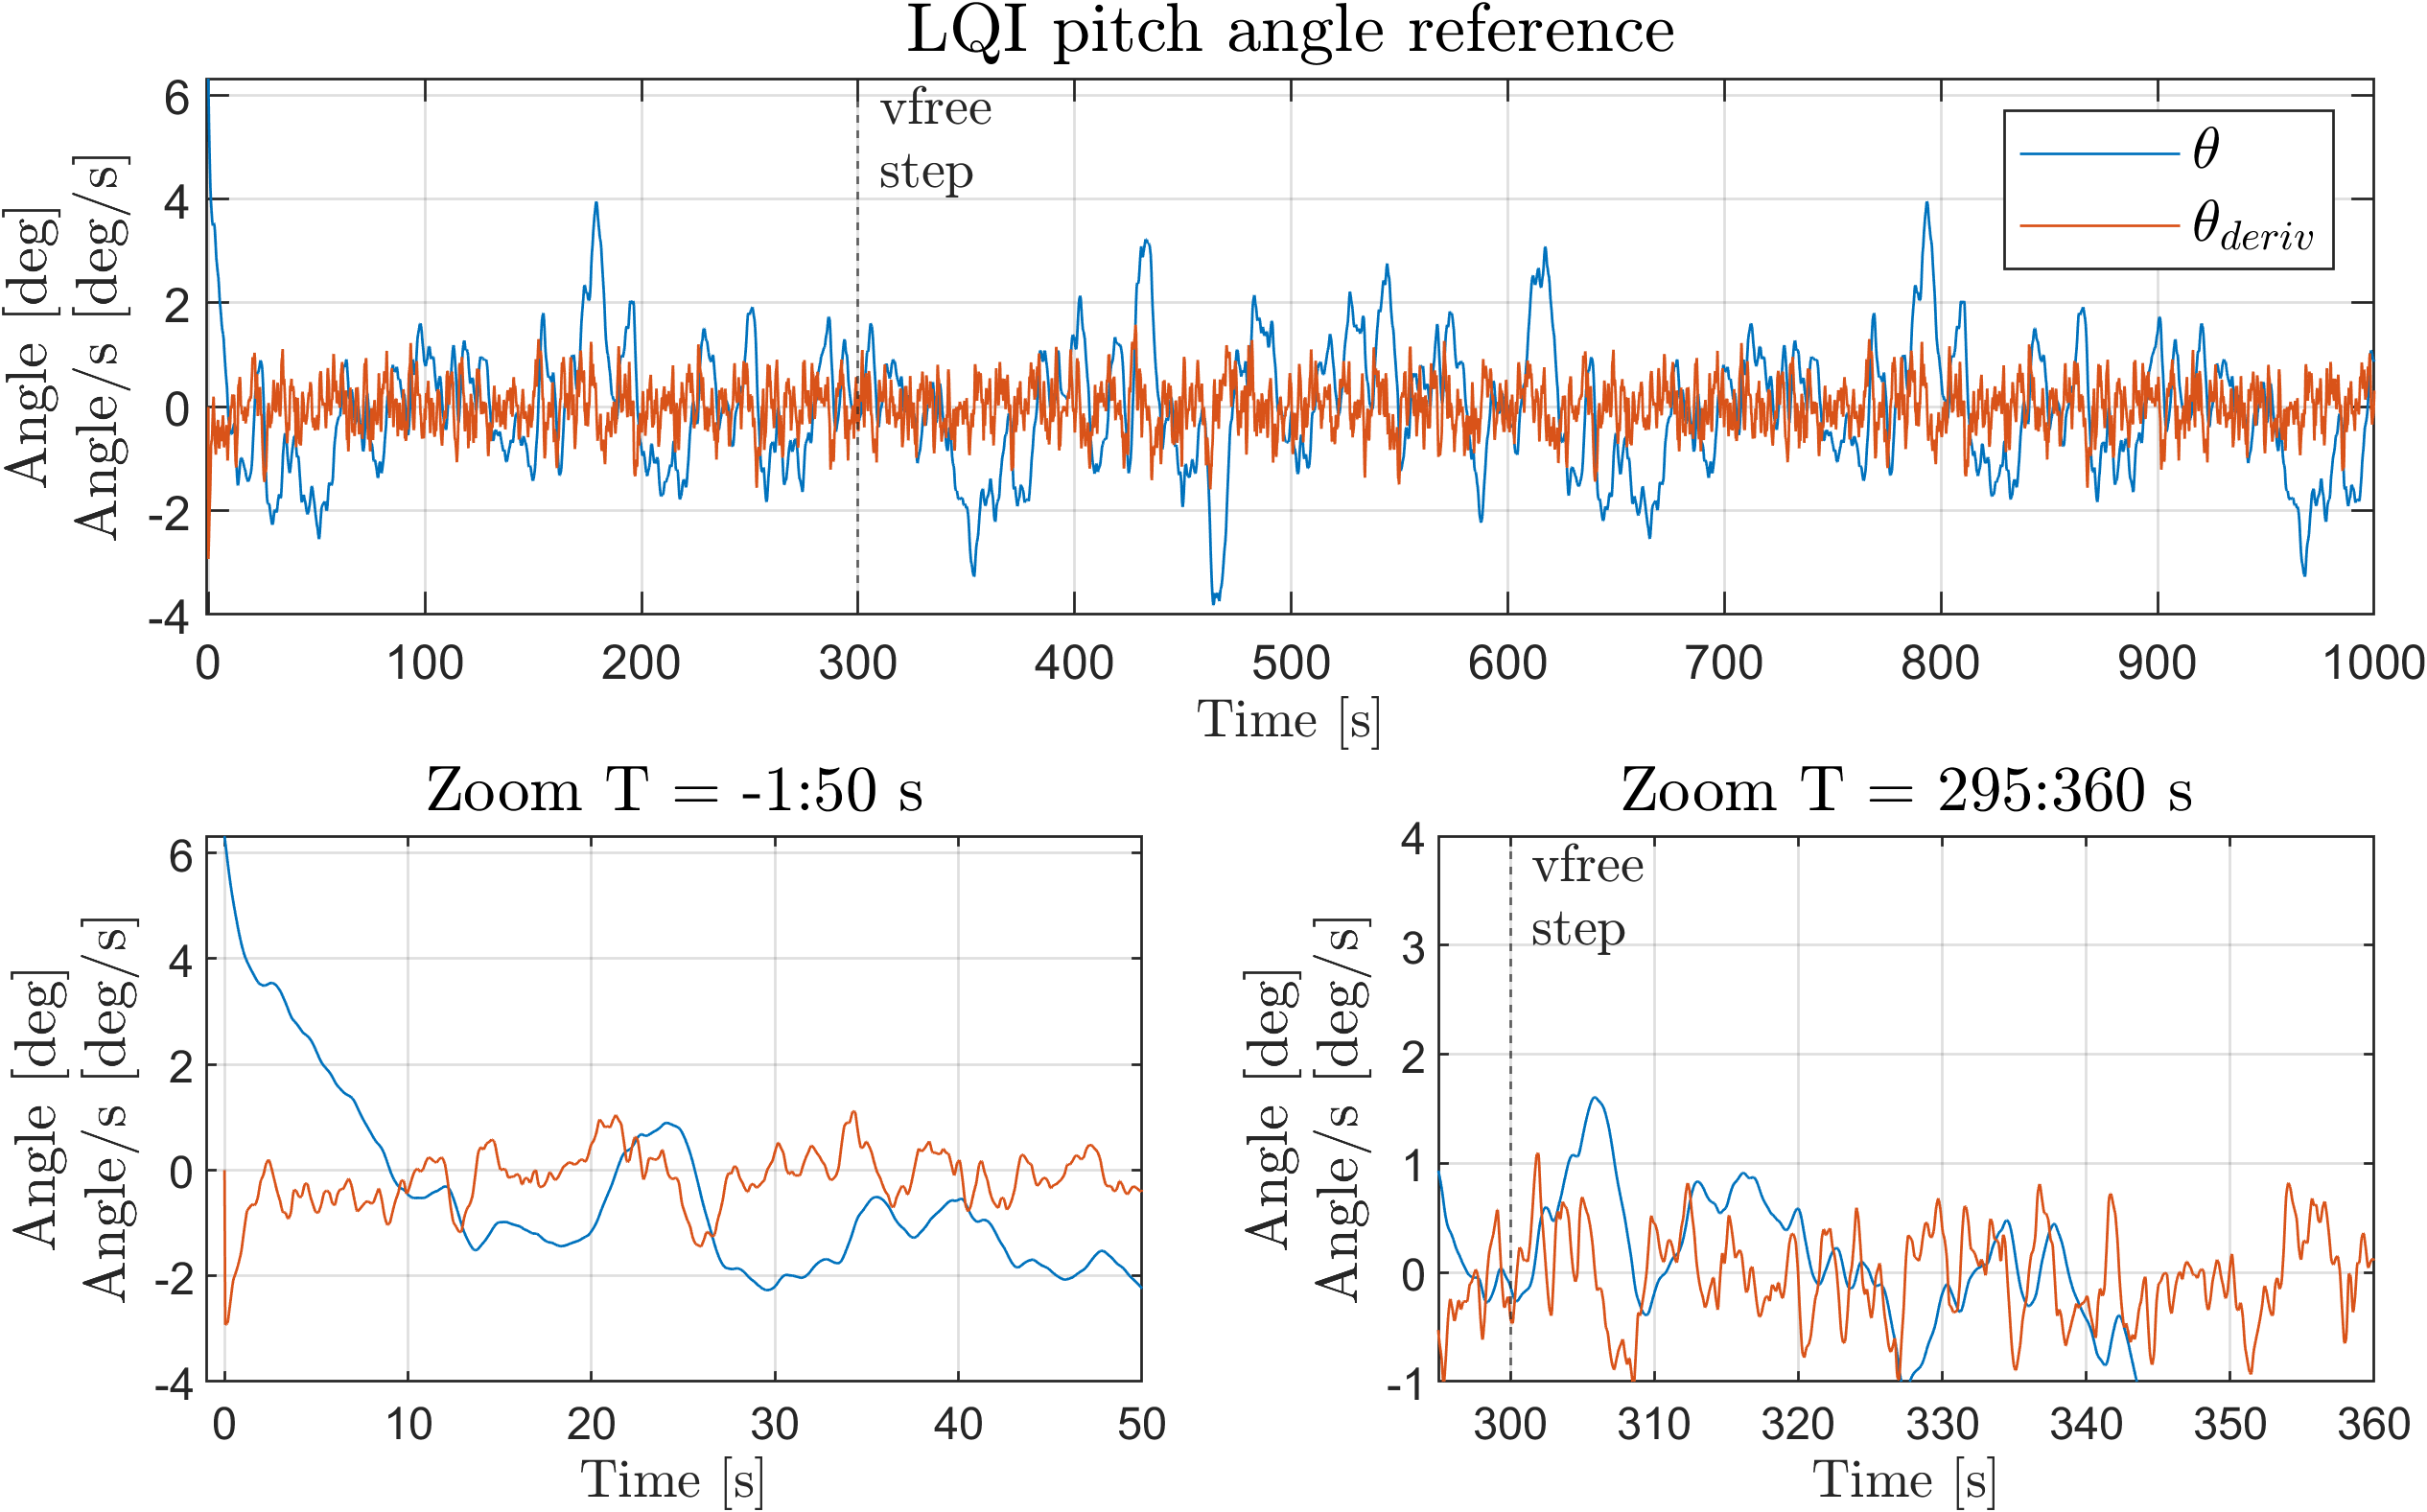
\includegraphics[width=0.7\linewidth]{Graphics/TestResults/linearModPerf/sim_01_pitch.png}
%	\caption{Simulink simulation results. Bottom left and right plots are zommed in at 0 to 50 s and 295 to 360 s.}
%	\label{fig:sim_01_pitch}
%\end{figure}